\chapter{\Coq{} Integrated Development Environment}
%\label{Addoc-coqide}
\ttindex{coqide}

The \Coq{} Integrated Development Environment is a graphical tool, to
be used as a user-friendly replacement to \texttt{coqtop}. Its main
purpose is to allow the user to navigate forward and backward into a
\Coq{} vernacular file, executing corresponding commands or undoing
them respectively. CREDITS ? Proof general, lablgtk, ...

\coqide{} is run by typing the command \verb|coqide| on the command
line. Without argument, the main screen is displayed with an ``unnamed
buffer'', and with a file name as argument, another buffer displaying
the contents of that file. Additionally, coqide accepts the same
options as coqtop, given in Chapter~\ref{Addoc-coqc}, the ones having
obviously no meaning for \coqide{} being ignored.

\begin{figure}[t]
\begin{center}
\ifx\pdftexversion\undefined   % si on est pas en pdflatex
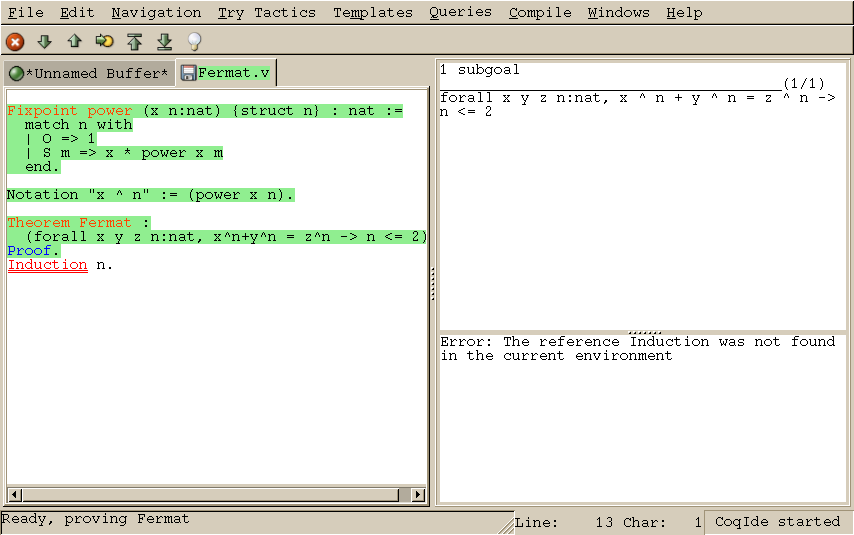
\includegraphics[width=1.0\textwidth]{coqide.eps}
\else
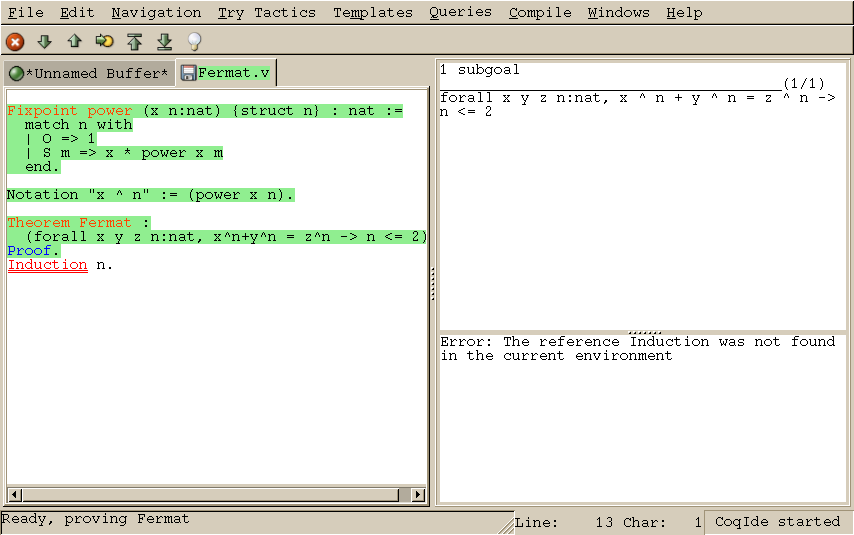
\includegraphics[width=1.0\textwidth]{coqide.png}
\fi
\end{center}
\caption{Coqide main screen}
\label{fig:coqide}
\end{figure}

\coqide{} main screen is shown on Figure~\ref{fig:coqide}.  (Attention
il manque la toolbar sur cet ecran car je l'ai enleve par defaut) At
the top is a menu bar, the left window is displaying the various
buffers, the upper right window is the ``goal window'', where goals to
prove are displayed. The lower right window is the ``message window'',
where various messages resulting from commands are displayed. At the
bottom is the status bar.

\section{The \texttt{File} menu}

Open/Create

Save

Save as

Save all

Revert All Buffers

Close Buffer

Print

Export to

Rehighlight

Quit

\section{The \texttt{Edit} menu}


\section{The \texttt{Navigation} menu}

Remplacer forward to et backward to par goto ?
idem pour la toolbar

\section{The \texttt{Try Tactics} menu}

Is it useful ?

\section{The \texttt{Templates} menu}

Need update to V8 syntax

\section{The \texttt{Commands} menu}

\section{The \texttt{Externals} menu}

\section{The \texttt{Configuration} menu}

\section{The \texttt{Help} menu}


% $Id$ 

%%% Local Variables: 
%%% mode: latex
%%% TeX-master: "Reference-Manual"
%%% End: 
